\documentclass[a4paper, 12pt]{article}
\usepackage[top=2cm, bottom=2cm, left=2.5cm, right=2.5cm]{geometry}
\usepackage[utf8]{inputenc}
\usepackage[brazilian]{babel}
\usepackage{indentfirst}
\usepackage{graphicx}
\usepackage{wrapfig}
\usepackage[pdftex]{hyperref}
\usepackage{amsmath}
\usepackage{subcaption}

\begin{document}
	\begin{center} %centralizar o texto abaixo
		{\Large Resposta de sistemas de primeira e segunda ordem por Laplace}\\[0.4cm]
		{\large Erik Yuji Goto}\\[0.2cm]
		{\normalsize RA: 234009}
	\end{center} %término do comando centralizar

\section{Resposta de sistemas de primeira e segunda ordem - Laplace com condições iniciais nulas}
\subsection{1ª equação - Solução analítica}
Queremos calcular a resposta ao degrau da seguinte equação diferencial
	\begin{equation}
		0.1\dot{y} + y = u
	\end{equation}
	\\Resolvendo a partir da transformada de Laplace temos:
	\begin{figure}[h]
		\center
		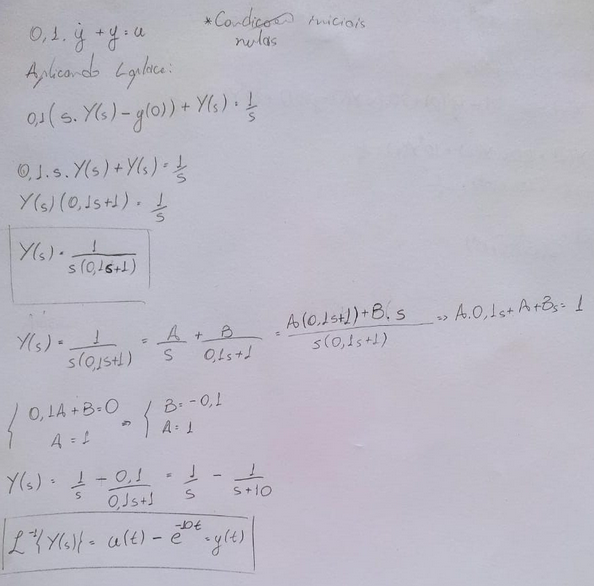
\includegraphics[scale=0.8]{Imagens/a.png}
		\caption{Analítica - Laplace}
	\end{figure}
\\Obtemos o seguinte gráfico ao plotar no Matlab:
	\begin{figure}[h]
		\center
		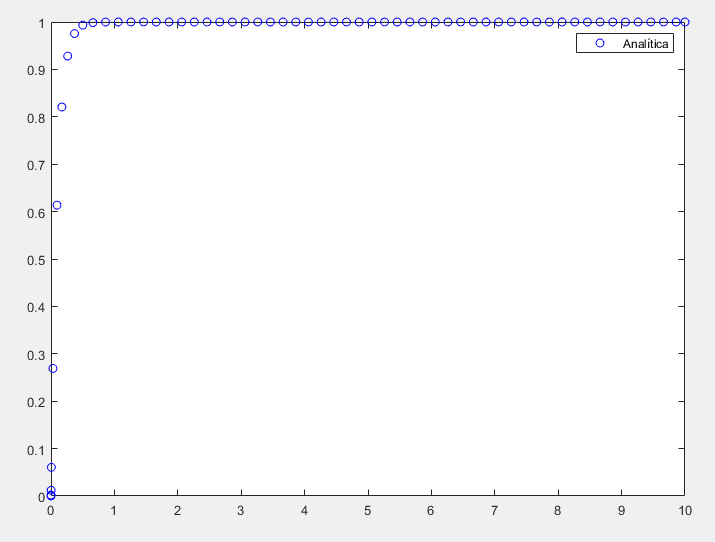
\includegraphics[scale=0.6]{Imagens/aaa.png}
		\caption{Gráfico resposta ao degrau}
	\end{figure}
	
	
	\newpage
\subsection{1ª equação - Solução simulink}
	A função transferência da equação é dada por $H(s) = \frac{Y(s)}{X(s)}$:
	\begin{figure}[h]
		\center
		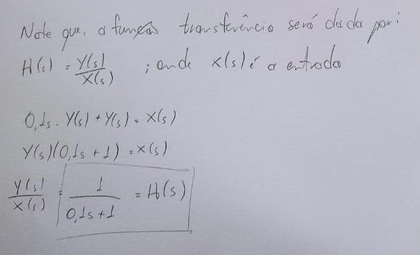
\includegraphics[scale=0.8]{Imagens/aa.png}
		\caption{Cáculo da função transferência}
	\end{figure}
	
	\begin{equation}
		H(s) = \frac{1}{0,1s + 1}
	\end{equation}
	\\No Simulink o diagrama de blocos com a função transferência fica da seguinte maneira:
	
	\begin{figure}[h]
	\centering
		\begin{subfigure}{.5\textwidth}
  			\centering
 			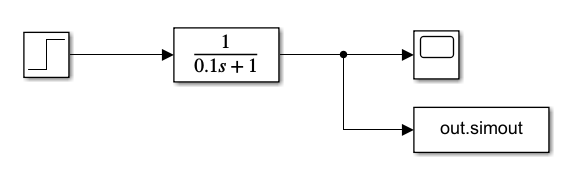
\includegraphics[scale=0.5]{Imagens/aaaa.png}
  			\caption{Diagrama de Blocos}
		\end{subfigure}%
		\begin{subfigure}{.5\textwidth}
  			\centering
  			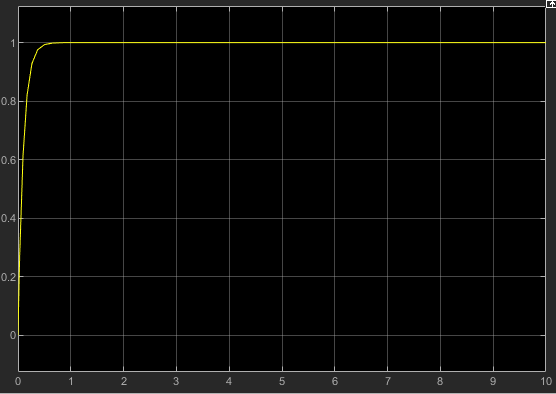
\includegraphics[scale=0.5]{Imagens/aaaaa.png}
  			\caption{Saída no Scope}
		\end{subfigure}
			\caption{Resolução no Simulink}
	\end{figure}
\newpage
\subsection{1ª equação - Analítica x Simulink}
	Vamos plotar as soluções analítica e pelo simulink para compará-las
	\begin{figure}[h]
		\centering
		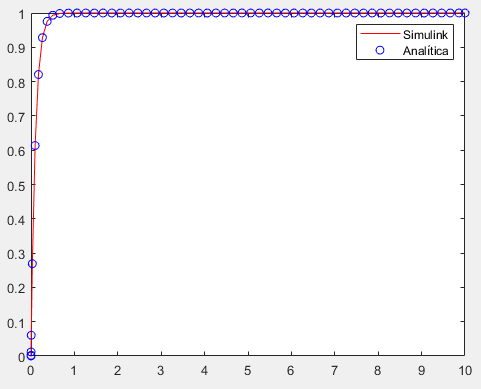
\includegraphics[scale=0.6]{Imagens/aaaaaa.png}
		\caption{Gráfico Analítica x Simulink}
	\end{figure}
	\begin{figure}[h]
		\centering
		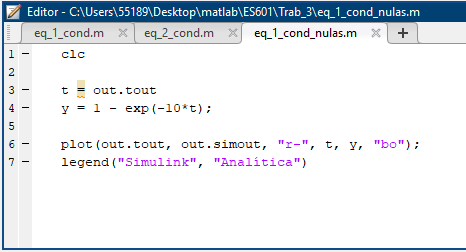
\includegraphics[scale=0.5]{Imagens/ppppp.png}
		\caption{Script Matlab}
	\end{figure}
	\\Conseguimos o mesmo plot para ambas as soluções, como era esperado.
	

%2ªequação
\newpage
\subsection{2ª equação - Solução analítica}
Queremos calcular a resposta ao degrau da seguinte equação diferencial
	\begin{equation}
		\ddot{y} + 20\dot{y} + 10^4y = u
	\end{equation}
	\\Resolvendo a partir da transformada de Laplace temos:
		\begin{center}
			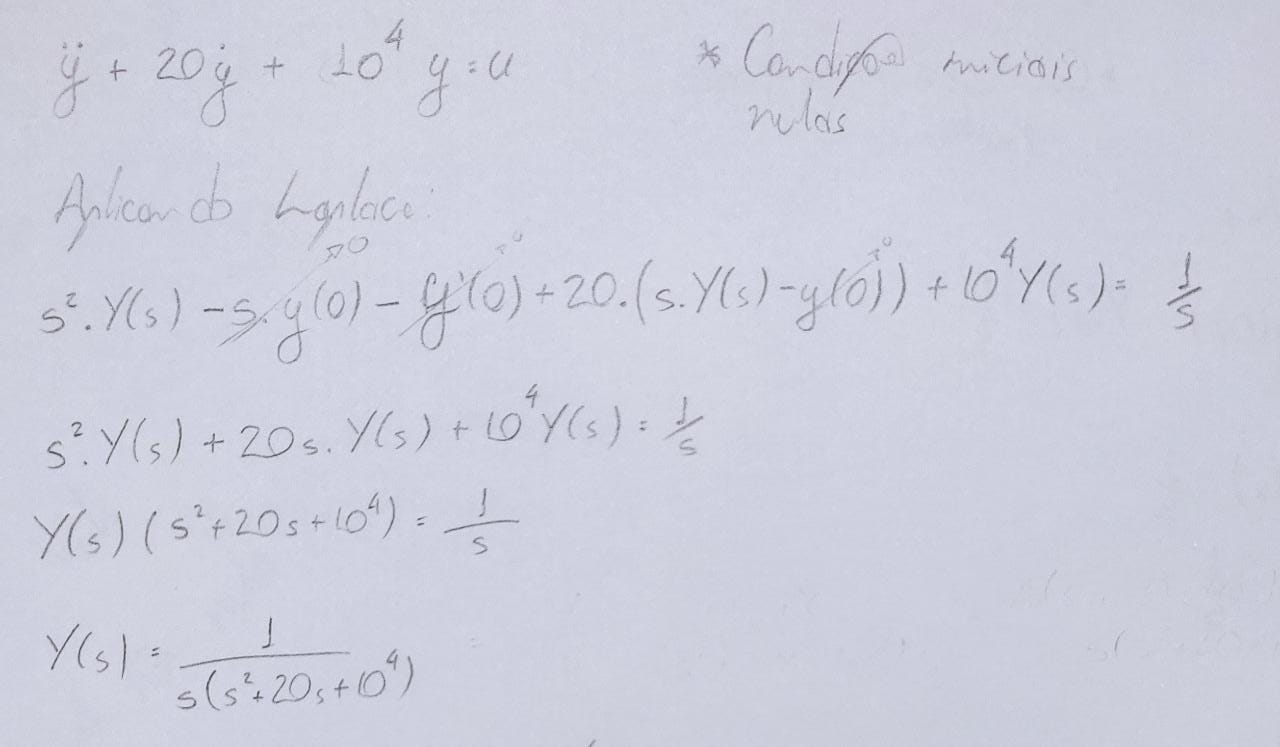
\includegraphics[scale=0.3]{Imagens/b.jpg}
			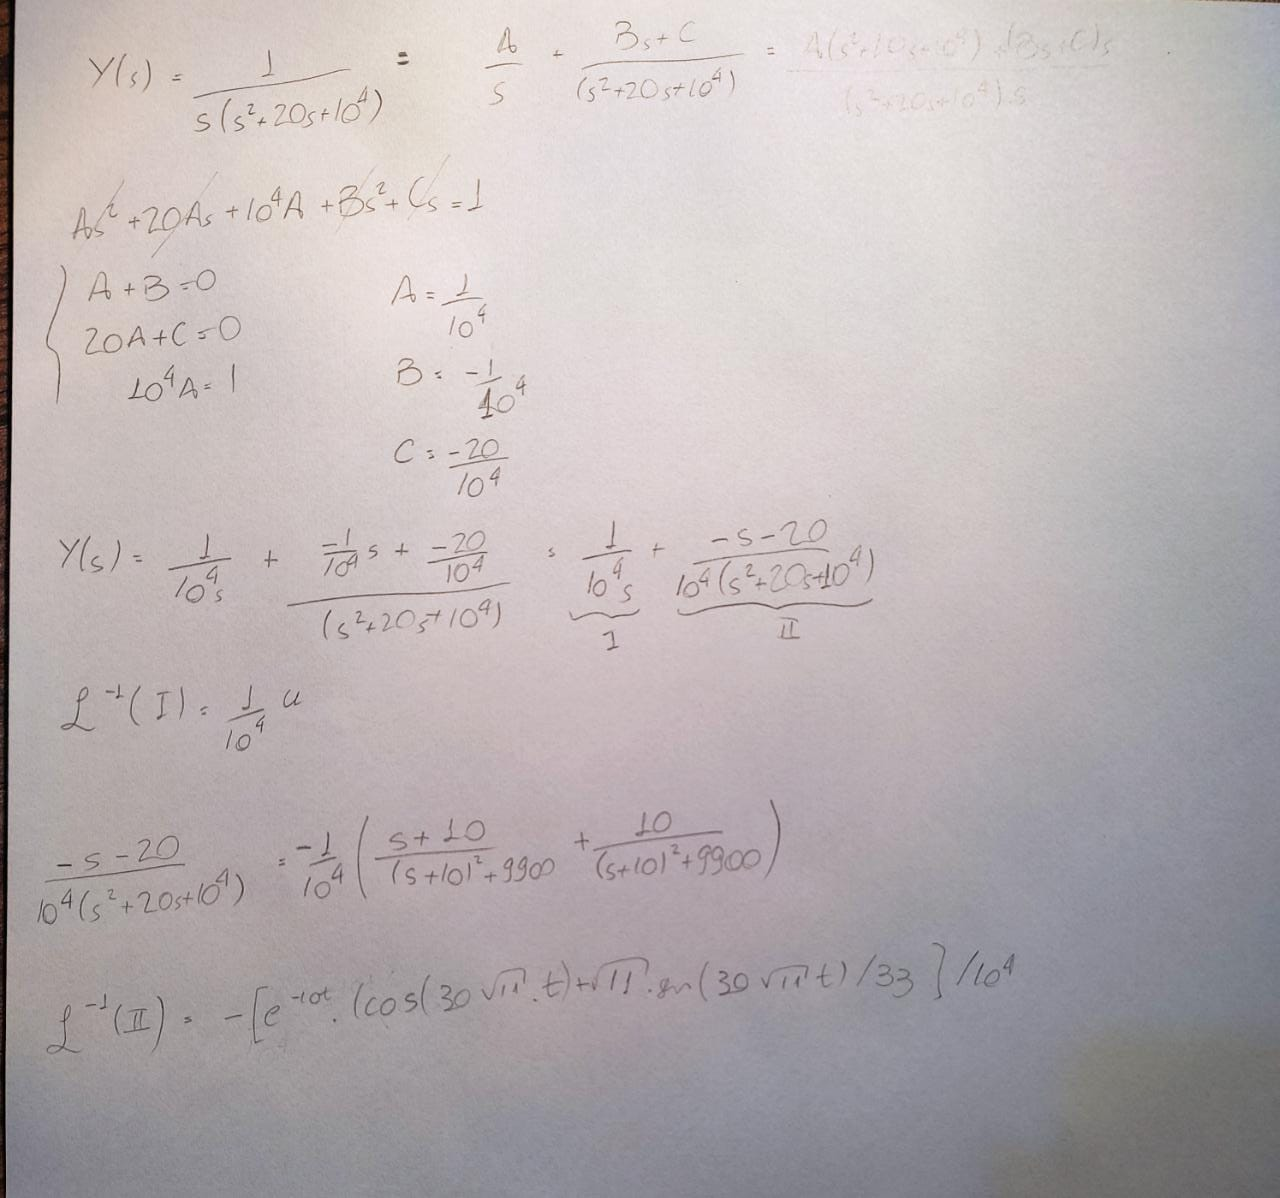
\includegraphics[scale=0.3]{Imagens/bb.jpg}
		\end{center}
		
	\begin{equation}
		y = 1/10000 - (exp(-10*t)*(cos(30*11^{1/2}*t) + (11^{1/2}*sin(30*11^{1/2}*t))/33))/10000;
	\end{equation}		
		
		
	Obtemos o seguinte gráfico ao plotar no Matlab:
	\begin{figure}[h]
		\center
		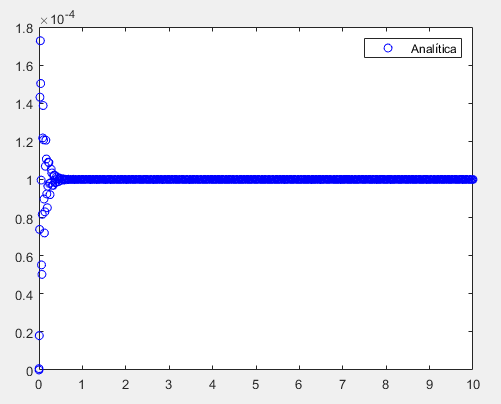
\includegraphics[scale=0.7]{Imagens/g.png}
		\caption{Gráfico resposta ao degrau}
	\end{figure}
	
	
	\newpage
\subsection{2ª equação - Solução simulink}
	A função transferência da equação é dada por $H(s) = \frac{Y(s)}{X(s)}$:
	\begin{figure}[h]
		\center
		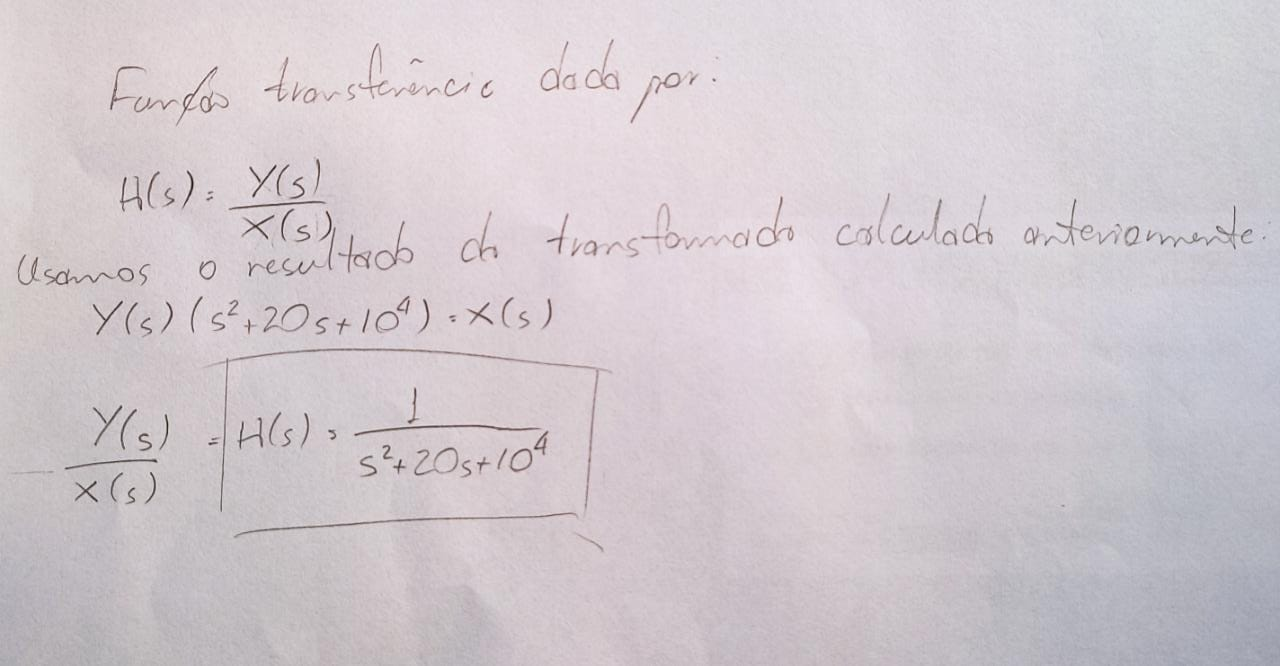
\includegraphics[scale=0.3]{Imagens/gg.jpg}
		\caption{Cáculo da função transferência}
	\end{figure}
	
	\begin{equation}
		H(s) = \frac{1}{s^2 + 20s + 10^4}
	\end{equation}
	\\No Simulink o diagrama de blocos com a função transferência fica da seguinte maneira:
	
	\begin{figure}[h]
	\centering
		\begin{subfigure}{.5\textwidth}
  			\centering
 			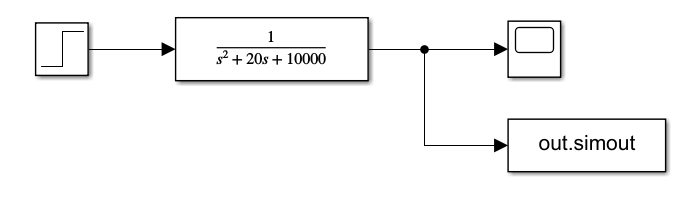
\includegraphics[scale=0.4]{Imagens/ggg.png}
  			\caption{Diagrama de Blocos}
		\end{subfigure}%
		\begin{subfigure}{.5\textwidth}
  			\centering
  			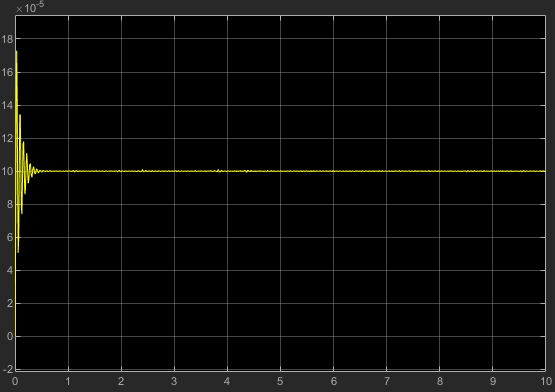
\includegraphics[scale=0.4]{Imagens/gggg.png}
  			\caption{Saída no Scope}
		\end{subfigure}
			\caption{Resolução no Simulink}
	\end{figure}
\newpage
\subsection{2ª equação - Analítica x Simulink}
	Vamos plotar as soluções analítica e pelo simulink para compará-las
	\begin{figure}[h]
		\centering
		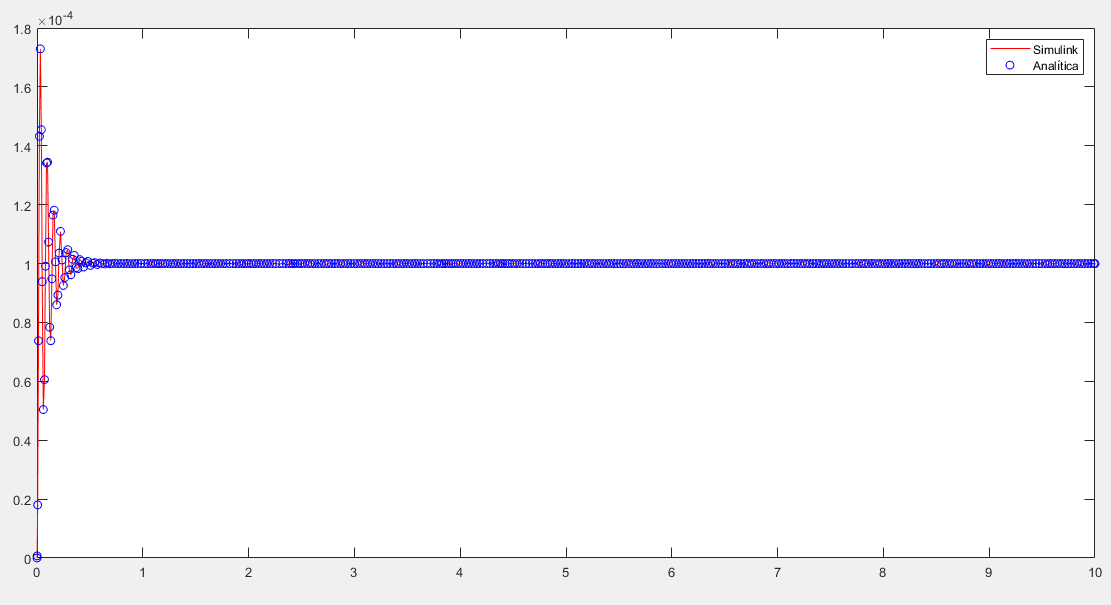
\includegraphics[scale=0.4]{Imagens/f.png}
		\caption{Gráfico Analítica x Simulink}
	\end{figure}
	\begin{figure}[h]
		\centering
		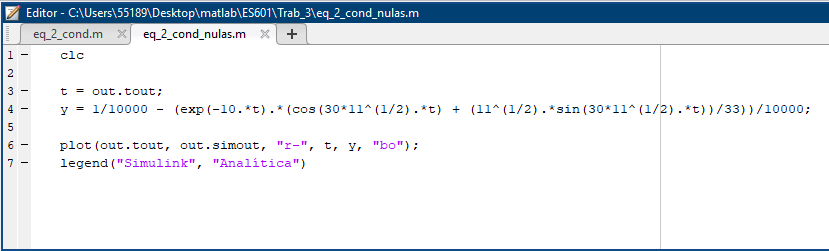
\includegraphics[scale=0.5]{Imagens/pp.png}
		\caption{Script Matlab}
	\end{figure}
	\\Conseguimos o mesmo plot para ambas as soluções, como era esperado.
	



\newpage
\section{Resposta de sistemas de primeira e segunda ordem - Com condições iniciais não nulas}

\subsection{1ª equação - Solução analítica}
Queremos calcular a resposta ao degrau da seguinte equação diferencial com condições iniciais não nulas:
	\begin{equation}
		0.1\dot{y} + y = u; y(0) = 10
	\end{equation}
	\\Resolvendo a partir da transformada de Laplace temos:
	\begin{figure}[h]
		\centering
		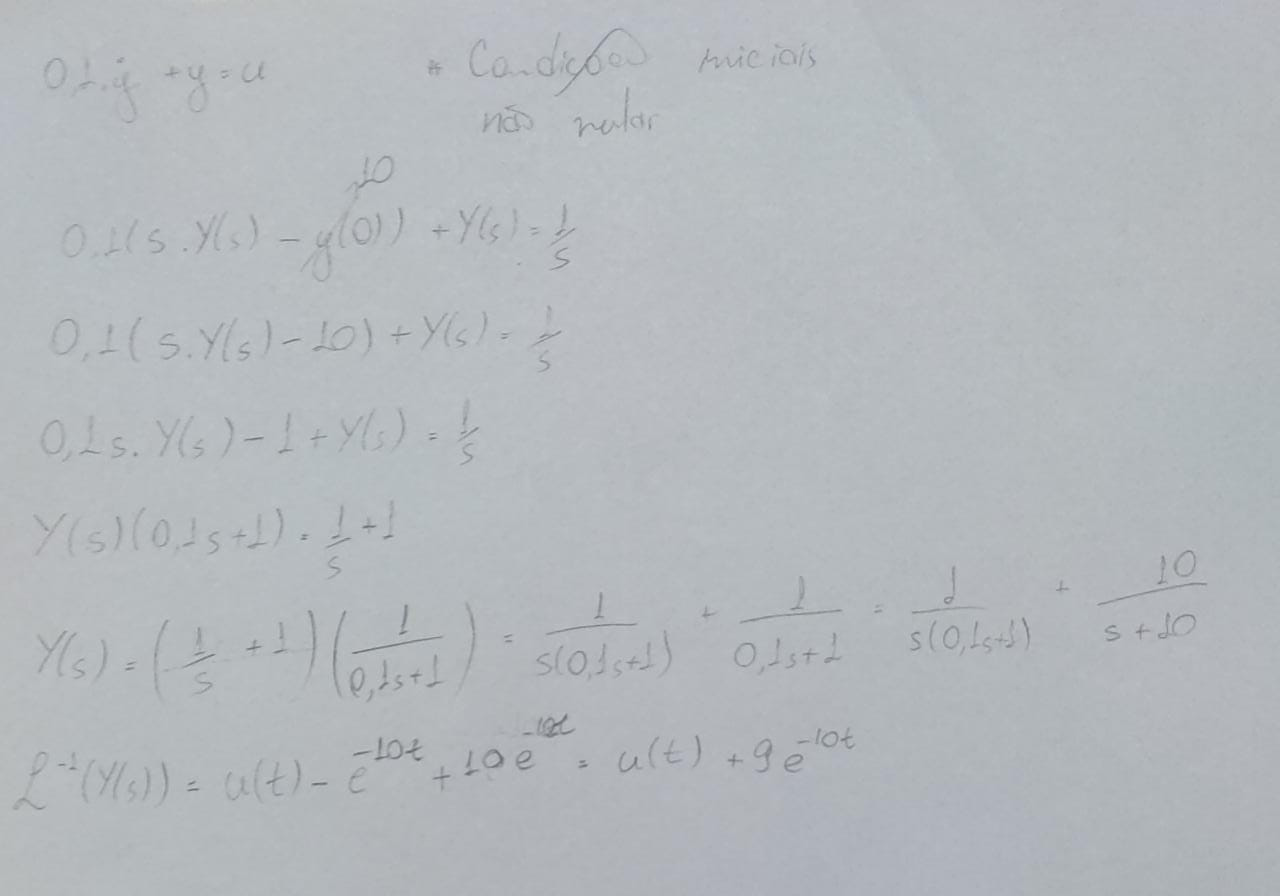
\includegraphics[scale=0.3]{Imagens/c.jpg}
		\caption{Condição Inicial não Nula}
	\end{figure}
		
	\begin{equation}
		y = u(t) + 9e^{-10t}
	\end{equation}		
		
		
	Obtemos o seguinte gráfico ao plotar no Matlab:
	\begin{figure}[h]
		\center
		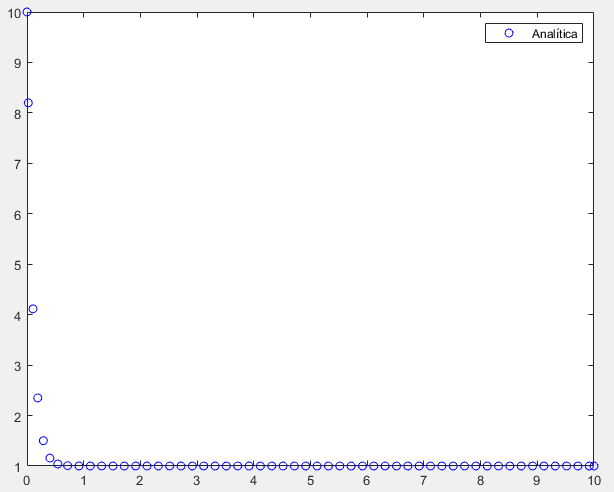
\includegraphics[scale=0.5]{Imagens/cc.png}
		\caption{Gráfico resposta ao degrau}
	\end{figure}
	
	
	\newpage
\subsection{1ª equação - Solução simulink}
	O diagrama de blocos construído no Simulink será:
	\begin{figure}[h]
	\centering
		\begin{subfigure}{.5\textwidth}
  			\centering
 			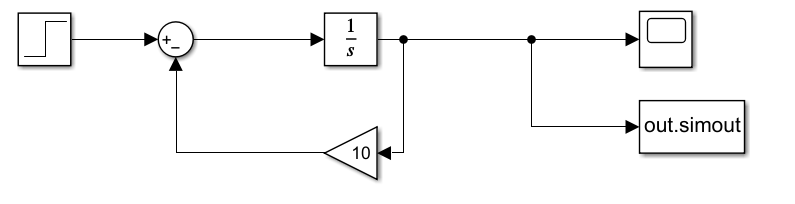
\includegraphics[scale=0.4]{Imagens/x.png}
  			\caption{Diagrama de Blocos}
		\end{subfigure}%
		\begin{subfigure}{.5\textwidth}
  			\centering
  			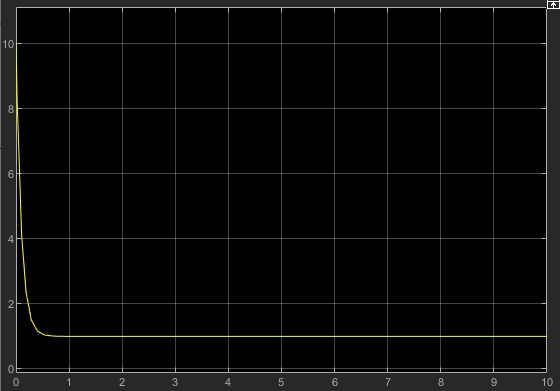
\includegraphics[scale=0.4]{Imagens/xx.png}
  			\caption{Saída no Scope}
		\end{subfigure}
			\caption{Resolução no Simulink}
	\end{figure}
	
\newpage
\subsection{1ª equação - Analítica x Simulink}
	Vamos plotar as soluções analítica e pelo simulink para compará-las
	\begin{figure}[h]
		\centering
		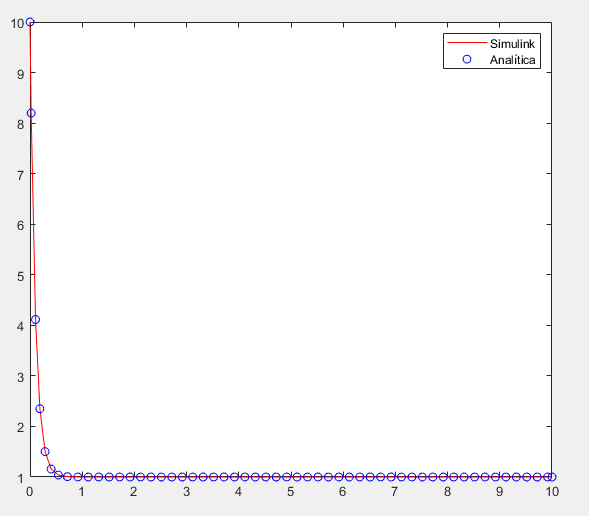
\includegraphics[scale=0.5]{Imagens/xxx.png}
		\caption{Gráfico Analítica x Simulink}
	\end{figure}
	\begin{figure}[h]
		\centering
		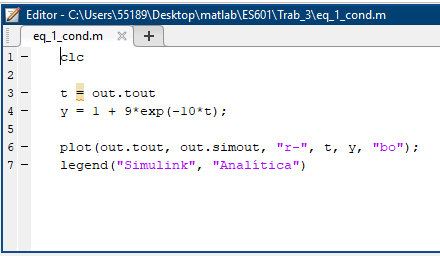
\includegraphics[scale=0.5]{Imagens/ppp.png}
		\caption{Script Matlab}
	\end{figure}
	\\Conseguimos o mesmo plot para ambas as soluções, como era esperado.
	




%2ªequação
\newpage
\subsection{2ª equação - Solução analítica}
Queremos calcular a resposta ao degrau da seguinte equação diferencial
	\begin{equation}
		\ddot{y} + 20\dot{y} + 10^4 = u; y(0) = 0, \dot{y}(0) = 10
	\end{equation}
	\\Resolvendo a partir da transformada de Laplace temos:
		\begin{center}
			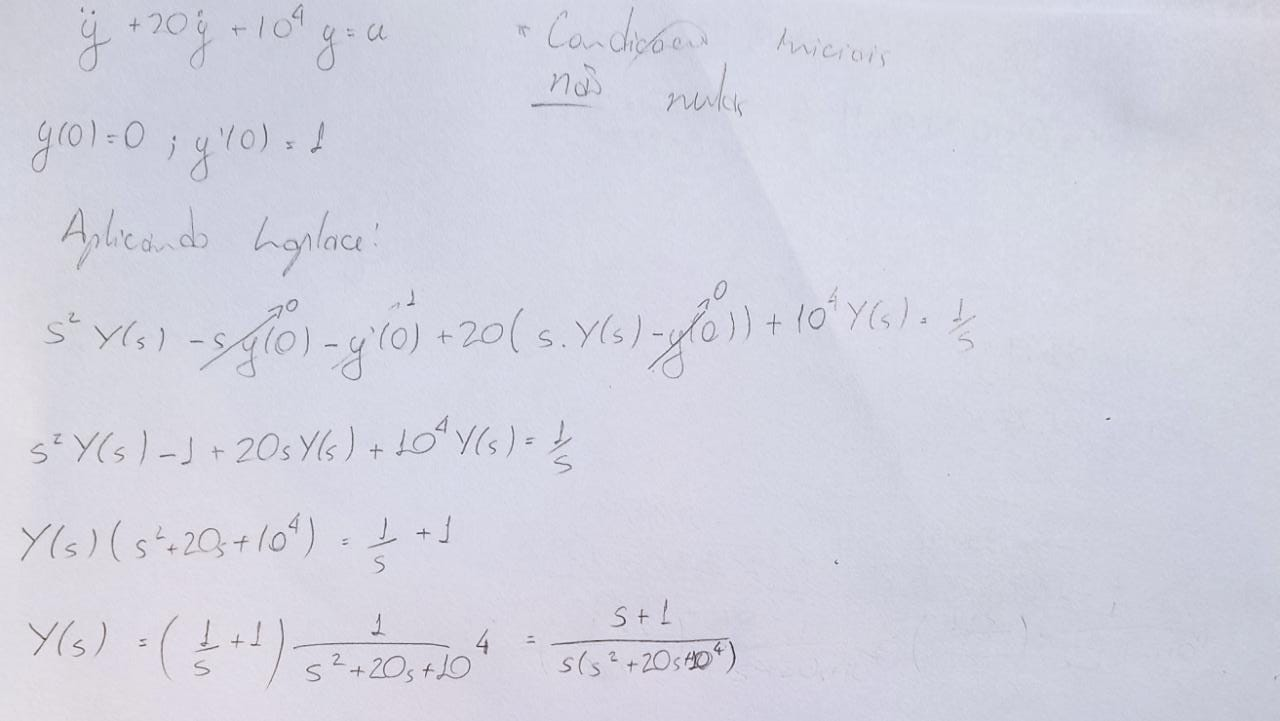
\includegraphics[scale=0.22]{Imagens/kk.jpg}
			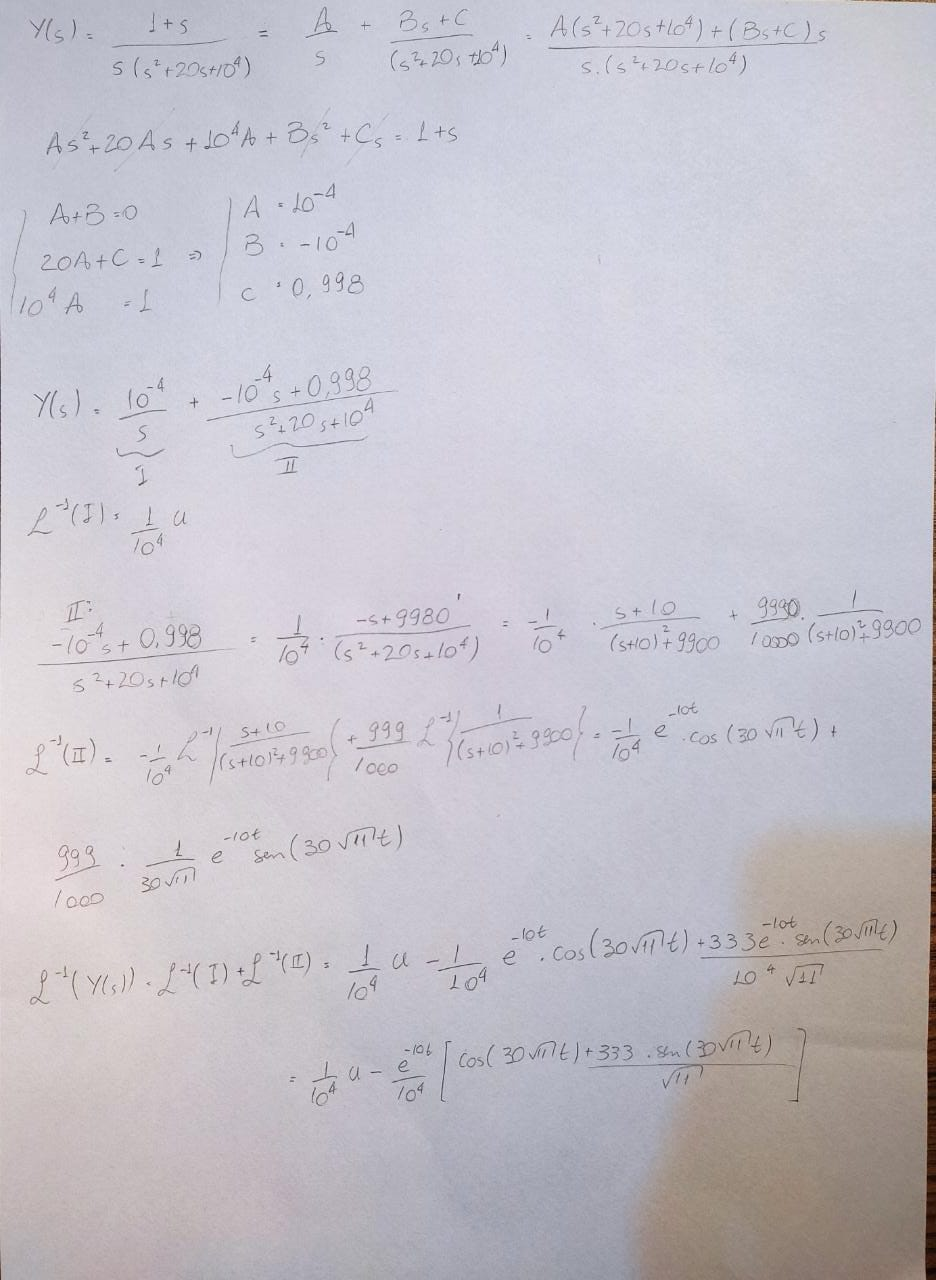
\includegraphics[scale=0.3]{Imagens/l.jpg}
		\end{center}
		
	\begin{equation}
		y = 1/10000 - (exp(-10*t)*(cos(30*11^{1/2}*t) - (333*11^{1/2}*sin(30*11^{1/2}*t))/11))/10000;
	\end{equation}		
		
		
	Obtemos o seguinte gráfico ao plotar no Matlab:
	\begin{figure}[h]
		\center
		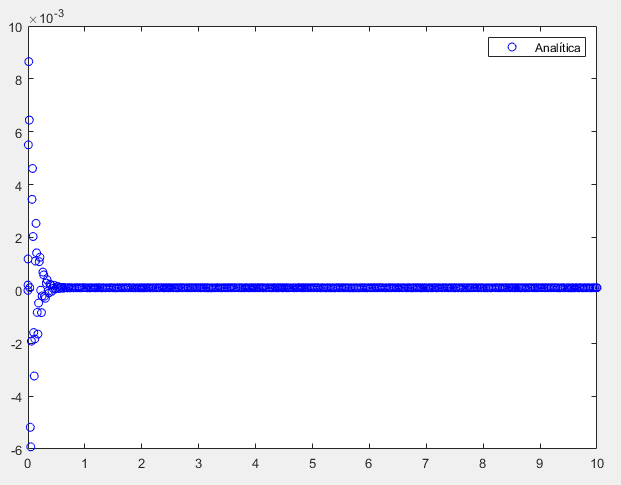
\includegraphics[scale=0.6]{Imagens/z.png}
		\caption{Gráfico resposta ao degrau}
	\end{figure}
	
	
	\newpage
\subsection{2ª equação - Solução simulink}
	A solução por diagrama de blocos é dado por:
	\begin{figure}[h]
	\centering
		\begin{subfigure}{.5\textwidth}
  			\centering
 			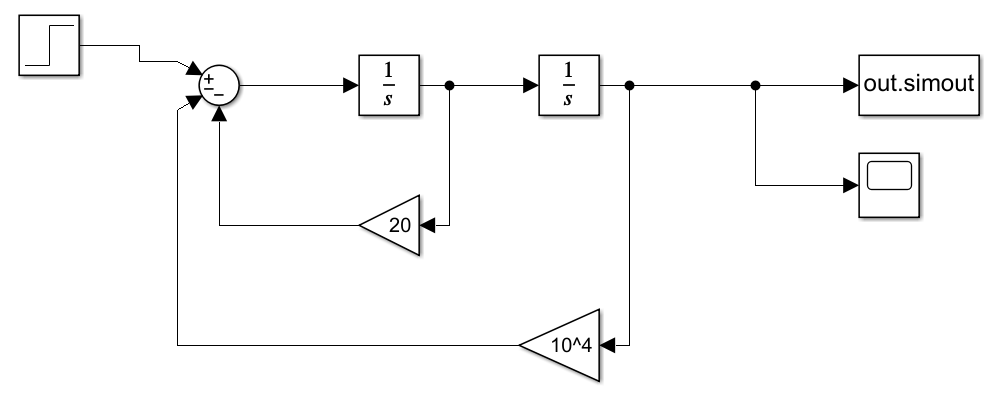
\includegraphics[scale=0.3]{Imagens/zz.png}
  			\caption{Diagrama de Blocos}
		\end{subfigure}%
		\begin{subfigure}{.5\textwidth}
  			\centering
  			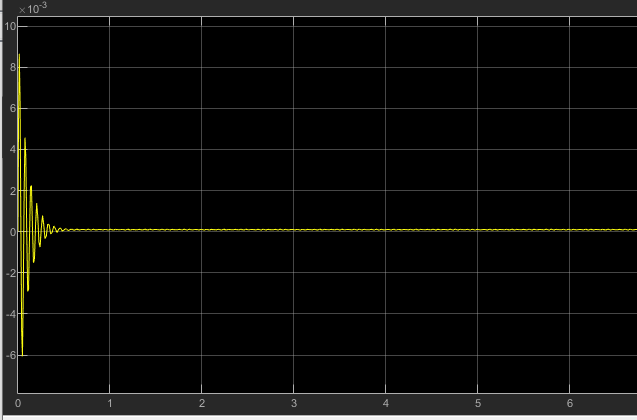
\includegraphics[scale=0.4]{Imagens/zzz.png}
  			\caption{Saída no Scope}
		\end{subfigure}
			\caption{Resolução no Simulink}
	\end{figure}
\newpage
\subsection{2ª equação - Analítica x Simulink}
	Vamos plotar as soluções analítica e pelo simulink para compará-las
	\begin{figure}[h]
		\centering
		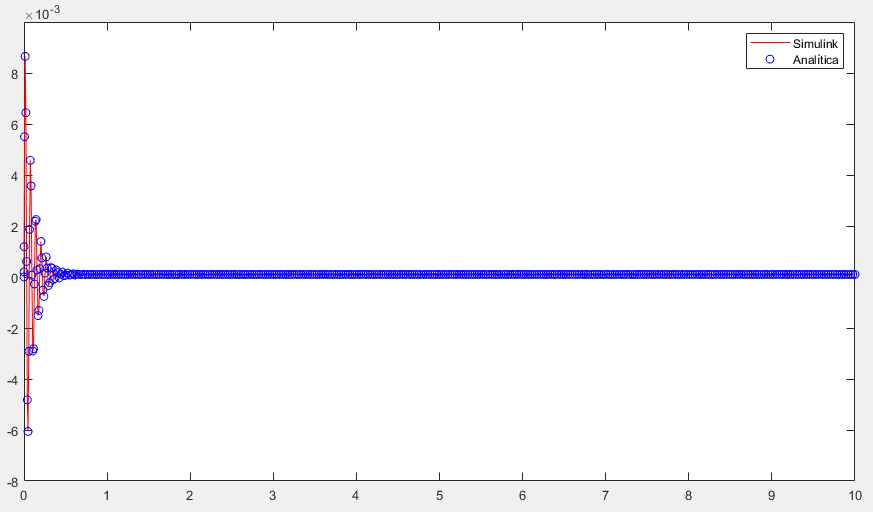
\includegraphics[scale=0.6]{Imagens/m.png}
		\caption{Gráfico Analítica x Simulink}
	\end{figure}
	\begin{figure}[h]
		\centering
		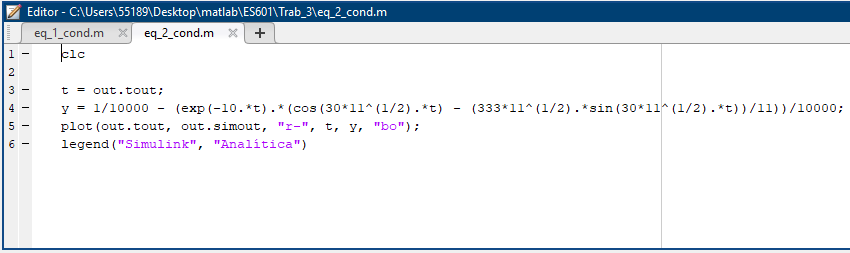
\includegraphics[scale=0.5]{Imagens/pppp.png}
		\caption{Script Matlab}
	\end{figure}
	\\Conseguimos o mesmo plot para ambas as soluções, como era esperado.
	


	
	
	
	
	
	
	
	
	
	
	
\end{document}